\documentclass {article}

\usepackage [utf8]{inputenc}
\usepackage {graphicx}
\usepackage {listings}
\usepackage [spanish]{babel}
\usepackage {color}

\lstdefinestyle{mystyle}{ 
    backgroundcolor=\color{white}, 
    commentstyle=\color{green}, 
    keywordstyle=\color{blue}, 
    basicstyle=\footnotesize\ttfamily,
    numbers=left,
    numberstyle=\tiny,
    frame=single,
    breaklines=true
}

\lstset{style=mystyle}

\author{Luis Fernando Torres Hernández}
\title{Practica 3: Algoritmo genético.}
\date{\today}
\def\description{Algoritmo genético.}

\makeatletter 
\def\@maketitle{ 
    \raggedright
    
\includegraphics[scale=0.5]{logo.png}\\[8ex] 
    \vspace{1.0cm}
\begin{center} {
    \Huge 
    \bfseries
    \sffamily \@title }\\[4ex] {\Large \@author}\\[4ex] 
    \@date\\[8ex]
    \vspace{1.0cm}
    \Large\description
    \newpage
\end{center}} 
\makeatother

\begin{document}
\maketitle


\section {Introducción}
En esta practica se desarrollo un algoritmo genético para optimizar
el diseño de armaduras planas usando un valor de peso como referencia.

En esta practica se hace un uso intensivo de apuntadores y memoria
dinámica, durante la ejecución se mantiene en memoria un arreglo de
cromosomas que representan posibles soluciones al problema.


\section {Desarrollo}
El código se dividio en 3 archivos de código fuente, el primero es 
\texttt{main.c} que contiene la función principal y el flujo de ejecución 
del programa, el segundo es \texttt{comun.c} que contiene funciones que 
son usadas en varias partes del código y el tercero es \texttt{comun.h} que 
contiene las definiciones de estructuras y prototipos de funciones que se usan en
\texttt{main.c} y \texttt{comun.c}.

Se utilizaron 2 estructuras, la primera es \texttt{instancia} que contiene los datos
de la instancia del problema, estos son la probabilidad de mutación, la probabilidad 
de cruce, el peso máximo permitido, el numero de elementos de los que se puede formar
la armadura y un arreglo de elementos que contiene el area y longitud de cada elemento.

La segunda estructura es \texttt{cromosoma} que contiene un genotipo que es un número
entero de 64 bits que representa la selección de elementos que forman la armadura,
el peso de la armadura y la aptitud que es un valor que indica que tan buena es la 
solución representada por el cromosoma, este valor se calcula como 
$$ \frac{1}{1000 * \left\|M-P\right\|} $$
donde $M$ es el peso máximo permitido y $P$ es el peso de la armadura representada 
por el cromosoma. El código se puede ver en la Figura \ref{fig:structs}.

\begin{figure}[htbp]
    \centering
    \begin{lstlisting}[language=C]
typedef struct instancia{
    float p_cruza;
    float p_mutacion;
    float maxima;
    int n_objetos;
    float *area;
    float *longitud;
} instancia;

typedef struct cromosoma{
    long long int genotipo;
    float peso;
    float aptitud;
} cromosoma;
    \end{lstlisting}
    \caption{Definición de estructuras para la instancia y el cromosoma}
    \label{fig:structs}
        
\end{figure}


\subsection{Algoritmo genético}
El algoritmo genético que se implemento en esta practica 
sigue los siguientes pasos:

\begin{itemize}
    \item Se genera una población inicial aleatoria.
    \item Se calcula la aptitud de cada cromosoma en la población.
    \item Se hace una selección de la siguiente generación de cromosomas.
    \item Se realiza el cruce de los cromosomas seleccionados.
    \item Se realiza la mutación de los cromosomas seleccionados.
    \item Se repiten los pasos 2 a 5 por un número determinado de iteraciones.
\end{itemize}

\subsubsection{Selección}
La selección de los cromosomas se realizo usando el método de ruleta,
este consiste en asignas a cada cromosoma un rango de valores proporcional a su aptitud,
luego se genera un número aleatorio y se selecciona el cromosoma cuyo rango contiene
ese número, este proceso se repite hasta seleccionar el número de cromosomas deseado
lo que se muestra en la Figura \ref{fig:seleccion}.

\begin{figure}[htbp]
    \centering
    \begin{lstlisting}[language=C]
cromosoma *seleccion(cromosoma *poblacion, int n) {
    cromosoma *seleccionado = malloc(sizeof(cromosoma)*n);
    float total_aptitud = 0.0;
    for (int i = 0; i < n; i++) {
        total_aptitud += poblacion[i].aptitud;
    }

    for (int i = 0; i < n; i++) {
        float r = ((float)rand() / RAND_MAX) * total_aptitud; 
        float acumulado = 0.0;
        for (int j = 0; j < n; j++) {
            acumulado += poblacion[j].aptitud;
            if (acumulado >= r) {
                copiar_cromosoma(&poblacion[j], &seleccionado[i]); 
                break;
            }
        }
    }
    return seleccionado;
}
    \end{lstlisting}
    \caption{Selección de cromosomas usando el método de ruleta}
    \label{fig:seleccion}   
\end{figure}

\subsubsection{Cruce}
La cruza se realizo usando el método de punto de cruce, este consiste en 
seleccionar un punto aleatorio en el genotipo y luego intercambiar los bits
de los cromosomas seleccionados a partir de ese punto usando una probabilidad 
de cruce, esto se muestra en la Figura \ref{fig:cruce}.

\begin{figure}[hbp]
    \centering
    \begin{lstlisting}[language=C]
void cruzar(cromosoma *padre1, cromosoma *padre2, float pc) {
    int punto_cruce = rand() % MAX_BITS;
    long long int mascara = (1LL << punto_cruce);
    while (mascara) {
        float probabilidad = (float)rand() / RAND_MAX;
        if (probabilidad < pc) {
            long long int bit1 = padre1->genotipo & mascara;
            long long int bit2 = padre2->genotipo & mascara;
            padre1->genotipo = (padre1->genotipo & ~mascara) | bit2;
            padre2->genotipo = (padre2->genotipo & ~mascara) | bit1;
        }
        mascara >>= 1;
    }
}
    \end{lstlisting}
    \caption{Cruce de cromosomas usando el método de punto de cruce}
    \label{fig:cruce}   
\end{figure}

\subsubsection{Mutación}
La mutación se realizo bajo el siguiente criterio, se genera un número 
aleatorio y si este es menor a la probabilidad de mutación se invierte 
el valor del bit correspondiente en el genotipo del cromosoma, esto se 
muestra en la Figura \ref{fig:mutacion}.

\begin{figure}[hbp]
    \centering
    \begin{lstlisting}[language=C]
void mutar(cromosoma *poblacion, int n, float pm) {
    for (int i = 0; i < n; i++) {
        long long int mascara = 1;
        for (int j = 0; j < MAX_BITS; j++) {
            float probabilidad = (float)rand() / RAND_MAX;
            if (probabilidad < pm) {
                poblacion[i].genotipo ^= mascara; // Cambia el bit correspondiente
            }
            mascara <<= 1;
        }
    }
}
    \end{lstlisting}
    \caption{Mutación de cromosomas usando el método de inversión de bits}
    \label{fig:mutacion}
\end{figure}

El programa permite seleccionar un archivo de datos que serán cargados
para hacer la optimización de la armadura y ejecuta el algoritmo genético 
por un número determinado de iteraciones, la ejecución se puede ver en la 
Figura \ref{fig:ejecucion}.

\begin{figure}[hbp]
    \centering
    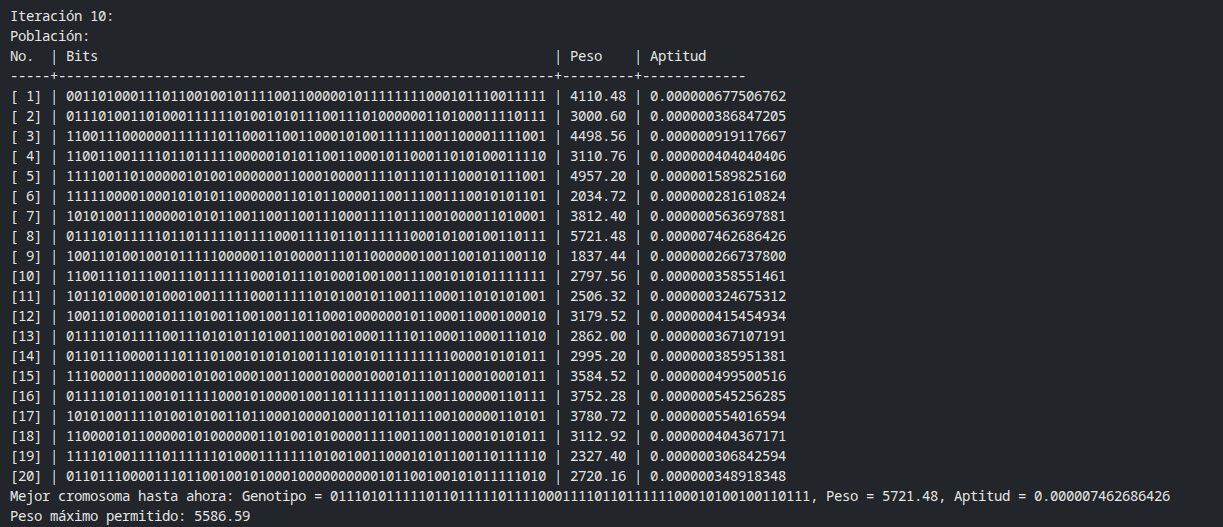
\includegraphics[scale=0.35]{ejecucion.png}
    \caption{Ejecución del programa}
    \label{fig:ejecucion}
\end{figure}


\end{document}